\documentclass[11pt, oneside]{article} 	% use "amsart" instead of "article" for AMSLaTeX format
\usepackage{geometry} 		% See geometry.pdf to learn the layout options. There are lots.
\geometry{letterpaper}  		% ... or a4paper or a5paper or ... 
\usepackage[parfill]{parskip} 		% Activate to begin paragraphs with an empty line rather than an indent
\usepackage{graphicx}				% Use pdf, png, jpg, or eps§ with pdflatex; use eps in DVI mode
								% TeX will automatically convert eps --> pdf in pdflatex		
\usepackage{amssymb}
\usepackage{amsmath}
\usepackage{authblk}
\usepackage[
backend=biber,
style=alphabetic,
]{biblatex}
\usepackage{graphicx}
\graphicspath{ {./images/} }
\usepackage{verbatim}
\usepackage{tikz} 
\usepackage{subcaption}
\captionsetup{compatibility=false}



\usepackage{syntonly}

% \syntaxonly \langle -- use this for checking syntax only
% \mbox {text} - keep together
% \fbox {text} - keep together and draw around

%\pagestyle{plain|headings|empty} % header and footer p.27
%SetFonts
%\include{filename}, \includeonly{filename1, filename2} , \input[fiename}

%SetFonts% 


\title{Dinosaur War: A Strategic Game of Utter Chance}
\author{Dave Fetterman}
\affil{Obviously Unemployed}
\date{3/2/23}
\begin{document}
\maketitle

\begin{abstract}

TODO 

\end{abstract}

\section{The Game}


\begin{figure}
\centering
\includegraphics[scale=.3]{cards}
\caption{Dinosaur Cards}
\end{figure}

\section{Dominance Score}

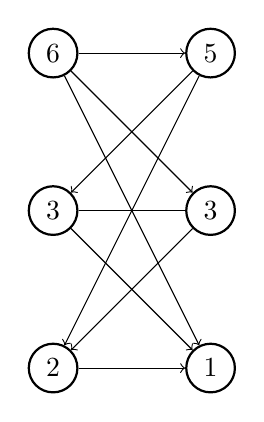
\begin{tikzpicture}
\begin{scope}[every node/.style={circle,thick,draw}]
    \node (1) at (0,0) {2};
    \node (2) at (0,2) {3};
    \node (3) at (0,4) {6};
    \node (4) at (2,0) {1};
    \node (5) at (2,2) {3};
    \node (6) at (2,4) {5};
\end{scope}

\draw[->] (1) -- (4); 
\draw[<-] (1) -- (5); 
\draw[<-] (1) -- (6); 
\draw[->] (2) -- (4); 
\draw[-] (2) -- (5); 
\draw[<-] (2) -- (6); 
\draw[->] (3) -- (4); 
\draw[->] (3) -- (5); 
\draw[->] (3) -- (6); 

\end{tikzpicture}

\section{Dominance in Dino Matrices}

$ \left[\begin{array}{cc}
                        &  \mathbf{5}\\ 
                        \mathbf{6} & 1\\
                      \end{array}\right] 
$

$ \left[\begin{array}{ccc}
                        & \mathbf{3} & \mathbf{5}\\ 
                       \mathbf{3} & 1 & 0\\
                        \mathbf{6} & 0 & 1\\
                      \end{array}\right] 
$

\begin{figure}
\centering
\begin{subfigure}{.5\textwidth}
  \centering
  
\[
\left[ 
\begin{array}{c@{}c@{}c@{}c}
& \mathbf{1} & \mathbf{3} & \mathbf{5} \\


\mathbf{2} &  \left[\begin{array}{ccc}
                        & \mathbf{3} & \mathbf{5}\\ 
                       \mathbf{3} & 1 & 0\\
                        \mathbf{6} & 0 & 1\\
                      \end{array}\right] 
                      & \left[\begin{array}{ccc}
                        & \mathbf{1} & \mathbf{5}\\ 
                       \mathbf{3} & 2 & 0 \\
                        \mathbf{6} & 0 & 2 \\
                      \end{array}\right]   
                      & \left[\begin{array}{ccc}
                        & \mathbf{1} & \mathbf{3}\\ 
                       \mathbf{3} & 2 & 1 \\
                        \mathbf{6} & 1 & 2 \\
                      \end{array}\right]   \\                      
                      
  \mathbf{3} & \left[\begin{array}{ccc}
                        & \mathbf{3} & \mathbf{5}\\ 
                        \mathbf{2} &0 & 0 \\
                        \mathbf{6} & 0 & 0 \\
                      \end{array}\right]
                      & \left[\begin{array}{ccc}
                        & \mathbf{1} & \mathbf{5}\\ 
                       \mathbf{2} & 2 & 0 \\
                        \mathbf{6} & 0 & 2 \\
                      \end{array}\right]   
                      & \left[\begin{array}{ccc}
                        & \mathbf{1} & \mathbf{3}\\ 
                       \mathbf{2} & 2 & 0 \\
                        \mathbf{6} & 0 & 2 \\
                      \end{array}\right]   \\                          
                      
                      
\mathbf{6} &  \left[\begin{array}{ccc}
                        & \mathbf{3} & \mathbf{5}\\ 
                       \mathbf{2} & -2 & -1 \\
                        \mathbf{3} & -1 & -2 \\
                      \end{array}\right] 
& \left[\begin{array}{ccc}
                        & \mathbf{1} & \mathbf{5}\\ 
                       \mathbf{2} & 0 & 0 \\
                        \mathbf{3} & 0 & 0 \\
                      \end{array}\right]   
                      & \left[\begin{array}{ccc}
                        & \mathbf{1} & \mathbf{3}\\ 
                       \mathbf{2} & 1 & 0 \\
                        \mathbf{3} & 0 & 1 \\
                      \end{array}\right]   \\    
\end{array}\right]
\]    
  \caption{Recursive game matrix}
\label{fig:236135_recursive}
\end{subfigure}

\begin{subfigure}{.5\textwidth}
\[
\left[ 
\begin{array}{c@{}c@{}c@{}c}
& \mathbf{1} & \mathbf{3} & \mathbf{5} \\


\mathbf{2} &  (\mathit{1} + .5 = 1.5) & (\mathit{-1} + 1 = 0) & (\mathit{-1} + 1.5 = .5) \\
\mathbf{3} &  (\mathit{1} +0 =  1) & (\mathit{0} + 1 = 1) & (\mathit{-1} + 1 = 0) \\                         
 \mathbf{6} & (\mathit{1} + -1.5 = -.5) & (\mathit{1} + 0 = 1) & (\mathit{1} + .5 = 1.5) \\
\end{array}\right]
\]    
\caption{Payoff matrix}
\label{fig:236135_payoff}
\end{subfigure}

\caption{$\{2,3,6\}$ vs. $\{1,3,5\}$}
\label{fig:236135}
\end{figure}




\begin{figure}
\centering
\begin{subfigure}{.5\textwidth}
  \centering
  
\[
\left[ 
\begin{array}{c@{}c@{}c@{}c}
& \mathbf{1} & \mathbf{3} & \mathbf{6} \\
\mathbf{2} &  \left[\begin{array}{ccc}
                        & \mathbf{3} & \mathbf{6}\\ 
                       \mathbf{3} & 0 & 0\\
                        \mathbf{6} & 0 & 0\\
                      \end{array}\right] 
                      & \left[\begin{array}{ccc}
                        & \mathbf{1} & \mathbf{6}\\ 
                       \mathbf{3} & 1 & 0 \\
                        \mathbf{6} & 0 & 1 \\
                      \end{array}\right]   
                      & \left[\begin{array}{ccc}
                        & \mathbf{1} & \mathbf{3}\\ 
                       \mathbf{3} & 2 & 1 \\
                        \mathbf{6} & 1 & 2 \\
                      \end{array}\right]   \\                      
                      
  \mathbf{3} & \left[\begin{array}{ccc}
                        & \mathbf{3} & \mathbf{6}\\ 
                        \mathbf{2} &-1 & 0 \\
                        \mathbf{6} & 0 & -1 \\
                      \end{array}\right]
                      & \left[\begin{array}{ccc}
                        & \mathbf{1} & \mathbf{6}\\ 
                       \mathbf{2} & 1 & 0 \\
                        \mathbf{6} & 0 & 1 \\
                      \end{array}\right]   
                      & \left[\begin{array}{ccc}
                        & \mathbf{1} & \mathbf{3}\\ 
                       \mathbf{2} & 2 & 0 \\
                        \mathbf{6} & 0 & 2 \\
                      \end{array}\right]   \\                          
                      
                      
\mathbf{6} &  \left[\begin{array}{ccc}
                        & \mathbf{3} & \mathbf{6}\\ 
                       \mathbf{2} & -2 & -1 \\
                        \mathbf{3} & -1 & -2 \\
                      \end{array}\right] 
& \left[\begin{array}{ccc}
                        & \mathbf{1} & \mathbf{6}\\ 
                       \mathbf{2} & 0 & 0 \\
                        \mathbf{3} & 0 & 0 \\
                      \end{array}\right]   
                      & \left[\begin{array}{ccc}
                        & \mathbf{1} & \mathbf{3}\\ 
                       \mathbf{2} & 1 & 0 \\
                        \mathbf{3} & 0 & 1 \\
                      \end{array}\right]   \\    
\end{array}\right]
\]    
  \caption{Recursive game matrix}
\label{fig:236136_recursive}
\end{subfigure}

\begin{subfigure}{.5\textwidth}
\[
\left[ 
\begin{array}{c@{}c@{}c@{}c}
& \mathbf{1} & \mathbf{3} & \mathbf{6} \\


\mathbf{2} &  (\mathit{1} + 0 = 1) & (\mathit{-1} + .5 = -.5) & (\mathit{-1} + 1.5 = .5) \\
\mathbf{3} &  (\mathit{1} -.5  =  .5) & (\mathit{0} + .5 = .5) & (\mathit{-1} + 1 = 0) \\                         
 \mathbf{6} & (\mathit{1} -1.5 = -.5) & (\mathit{1} + 0 = 1) & (\mathit{0} + .5 = .5) \\
\end{array}\right]
\]    
\caption{Payoff matrix}
\label{fig:236136_payoff}
\end{subfigure}

\caption{$\{2,3,6\}$ vs. $\{1,3,6\}$}
\label{fig:236136}
\end{figure}



\section{Pieceyard}



\begin{thebibliography}{9}
\bibitem{1}
Wikipedia: \url{https://en.wikipedia.org/wiki/Minimax_theorem}
\end{thebibliography}


\end{document}

